\documentclass[serif,12pt]{beamer}
\usepackage{amssymb}
\usepackage[backend=bibtex8]{biblatex}

\usepackage{mathtools}
\usepackage{pxfonts}
% Movie includes
\usepackage{movie15}
\usepackage{hyperref}

\mode<presentation>
{ \usetheme{Madrid}
  \usecolortheme{seagull} }
\usepackage{graphicx}

% remove institute from footer
\makeatletter
\setbeamertemplate{footline}
{
  \leavevmode%
  \hbox{%
    \begin{beamercolorbox}[wd=.5\paperwidth,ht=2.25ex,dp=1ex,center]{author in head/foot}%
      \usebeamerfont{author in head/foot}\insertshorttitle%~~\beamer@ifempty{\insertshortinstitute}{}{(\insertshortinstitute)}
    \end{beamercolorbox}%
    \begin{beamercolorbox}[wd=.5\paperwidth,ht=2.25ex,dp=1ex,right]{date in head/foot}%
      \usebeamerfont{date in head/foot}\insertshortdate{}\hspace*{2em}
      \insertframenumber{} / \inserttotalframenumber\hspace*{2ex} 
    \end{beamercolorbox}}%
  \vskip0pt%
}
\makeatother

% remove navigation symbols
\setbeamertemplate{navigation symbols}{}

\title{Diffusion with Discontinuous Galerkin Schemes}
\author{Eric Shi \and Ammar Hakim}
\date{}
\institute[http://www.ammar-hakim.org/sj] % (optional, aber oft nötig)
{
  Princeton Plasma Physics Laboratory, Princeton, NJ
}

\addbibresource{SeminarTalk.bib}
% \bibliography{SeminarTalk.bib}

\begin{document}

\begin{frame}
  \titlepage
\end{frame}

\begin{frame}{Outline}
  \tableofcontents
  % You might wish to add the option [pausesections]
\end{frame}

\begin{frame}
  \frametitle{Outline}
  \begin{itemize}
  \item Looked at the following equation:
    \begin{align*}
      g = \frac{\partial f}{\partial t}=& \frac{\partial^2 f}{\partial x^2}
    \end{align*}
  \item Explicit update formulas derived for approximating solution
    using piecewise linear basis functions:
    \begin{align*}
      u_h(x,t) = u_0 + \frac{x-x_j}{\Delta x / 2} u_1
    \end{align*}
  \item Von Neumann analysis to find eigenvalues
  \end{itemize}
\end{frame}

\begin{frame}
  \frametitle{Notation}
  \begin{align*}
    \lbrack u \rbrack = & u^+ - u^-\\
    \overline{u} = & \frac{u^+ + u^-}{2}\\
    u^{\pm} = & \lim_{\epsilon \to 0^\pm} u(x+\epsilon,t)
  \end{align*}
  To simplify analysis we use the shift operator and its inverse
  \begin{align*}
    T u(j) &= u(j+1) \\
    T^{-1} u(j) &= u(j-1)
  \end{align*}
\end{frame}

\section{Asymmetric LDG}
\begin{frame}
  \frametitle{Asymmetric Local DG (AS LDG)}
  \begin{align*}
    \frac{\partial w}{\partial x} + f =& 0,\; \frac{\partial g}{\partial x} + w = 0
  \end{align*}
  \begin{itemize}
  \item Two choices of fluxes:
    \begin{itemize}
    \item $\hat{f} = f^+$, $\hat{w} = w^-$\\
      \begin{center}
        $\frac{\partial}{\partial t}\left(\begin{array}{cc}u_0\\u_1
          \end{array}\right) = \frac{1}{\Delta x^2}\left(
          \begin{array}{cc}
            4T^{-1} -8+4 T & 2T^{-1}+2-4 T \\
            -12 T^{-1} +6+6 T & -6 T^{-1} -24-6 T
          \end{array}\right)\left(\begin{array}{c}
            u_0 \\
            u_1 
          \end{array}
        \right)$
      \end{center}
    \item $\hat{f} = f^-$, $\hat{w} = w^+$\\
      \begin{center}
        $\frac{1}{\Delta x^2}\left(
          \begin{array}{cc}
            4T^{-1} -8+4 T & 4T^{-1}-2-2 T \\
            -6 T^{-1} -6+12 T & -6 T^{-1} -24-6 T
          \end{array}
        \right)$
      \end{center}
    \end{itemize}
  \end{itemize}
\end{frame}

\begin{frame}
  \frametitle{AS LDG Eigenvalues}
  \begin{itemize}
  \item Both choices of fluxes result in the same eigenvalues for the Von Neumann analysis
  \item Defining $x = k\Delta x$,
    \begin{align*}
      \lambda_1 = & \frac{1}{\Delta x^2}\left(-16 - 2 \cos x - \sqrt{186 + 136 \cos x + 2 \cos 2x}\right)\\
      \lambda_2 = & \frac{1}{\Delta x^2}\left(-16 - 2 \cos x + \sqrt{186 + 136 \cos x + 2 \cos 2x}\right)
    \end{align*}
  \item $k << 1$ limit:
    \begin{align*}
      \lambda_1 = & -\frac{36}{\Delta x^2} + 3 k^2 - \frac{k^4\Delta x^2}{6} + \frac{k^6\Delta x^4}{270} + O[k^7\Delta x^5]\\
      \lambda_2 = & -k^2 + \frac{k^6\Delta x^4}{540} + O[k^7\Delta x^5]
    \end{align*}
  \end{itemize}
\end{frame}

\section{Symmetric LDG}
\begin{frame}
  \frametitle{Symmetric Local DG (S LDG)}
  \begin{itemize}
  \item By averaging the results from the two AS LDG schemes, we get a symmetric scheme for LDG\\
    \begin{center}
      $\frac{1}{\Delta x^2}\left(
        \begin{array}{cc}
          4T^{-1} -8+4 T & 3T^{-1}-3 T \\
          -9 T^{-1} +9 T & -6 T^{-1} -24-6 T
        \end{array}
      \right)$
    \end{center}
  \item Defining $x = k\Delta x$,
    \begin{align*}
      \lambda_1 = & \frac{1}{\Delta x^2}\left(-16 - 2 \cos x - 2 \sqrt{42 + 40 \cos x - \cos 2x}\right)\\
      \lambda_2 = & \frac{1}{\Delta x^2}\left(-16 - 2 \cos x - 2 \sqrt{42 + 40 \cos x - \cos 2x}\right)
    \end{align*}
  \item $k << 1$ limit:
    \begin{align*}
      \lambda_1 = & -\frac{36}{\Delta x^2} + 3 k^2 - \frac{k^4\Delta x^2}{12} + O[k^6\Delta x^4]\\
      \lambda_2 = & -k^2 - \frac{k^4\Delta x^2}{12} +  O[k^6\Delta x^4]
    \end{align*}
  \end{itemize}
\end{frame}

\section{Direct DG}
\begin{frame}
  \frametitle{Direct DG (DDG)}
  \begin{itemize}
  \item We looked at two versions of Direct DG, the standard asymmetric version with interface corrections (DDG) and a symmetric version (SDDG)
  \item DDG solves the following weak form:
    \begin{align*}
      \int_{I_j} u_t v \mathrm{d}x -\widehat{(u_x)}v\bigr|_{x_{j-\frac{1}{2}}}^{x_{j+\frac{1}{2}}}+\int_{I_j} u_x v_x \mathrm{d}x+ \frac{1}{2}\lbrack u\rbrack(v_x)_{j+\frac{1}{2}}^- + \frac{1}{2}\lbrack u\rbrack(v_x)_{j-\frac{1}{2}}^+= & 0
    \end{align*}
  \item The flux is defined as:
    \begin{align*}
      \widehat{u_x} = & \beta_0 \frac{\lbrack u \rbrack}{\Delta x} + \overline{u_x} + \beta_1 \Delta x \lbrack u_{xx} \rbrack
    \end{align*}
  \item For $k=1$, took $\beta_0 = 2$ and $\beta_1 = 0$
  \end{itemize}
\end{frame}

\begin{frame}
  \frametitle{DDG Scheme}
  \begin{itemize}
  \item Obtained the following update formulas:\\
    \begin{center}
      $\frac{1}{\Delta x^2}\left(
        \begin{array}{cc}
          2T^{-1} -4+2 T & T^{-1}- T \\
          -3 T^{-1} +3 T & -12
        \end{array}
      \right)$
    \end{center}
  \item Defining $x = k\Delta x$,
    \begin{align*}
      \lambda_1 = & \frac{1}{\Delta x^2}\left(-8 + 2 \cos x - 2 \sqrt{6 + 4 \cos x - \cos 2x}\right)\\
      \lambda_2 = & \frac{1}{\Delta x^2}\left(-8 + 2 \cos x + 2 \sqrt{6 + 4 \cos x - \cos 2x}\right)
    \end{align*}
  \item $k << 1$ limit:
    \begin{align*}
      \lambda_1 = & -\frac{12}{\Delta x^2} - k^2 + \frac{k^4\Delta x^2}{4} + O[k^6\Delta x^4]\\
      \lambda_2 = & -k^2 - \frac{k^4\Delta x^2}{12} + \frac{k^6 \Delta x^4}{40} + O[k^7\Delta x^5]
    \end{align*}
  \end{itemize}
\end{frame}

\section{Symmetric Direct DG}
\begin{frame}
  \frametitle{Symmetric DDG (SDDG)}
  \begin{itemize}
  \item SDDG solves the following weak form:
    \begin{align*}
      \int_{I_j} u_t v \mathrm{d}x -\widehat{(u_x)}v\bigr|_{x_{j-\frac{1}{2}}}^{x_{j+\frac{1}{2}}}+\int_{I_j} u_x v_x \mathrm{d}x+ (\lbrack u\rbrack\widehat{v_x})_{j+\frac{1}{2}}^- + (\lbrack u\rbrack \widehat{v_x} )_{j-\frac{1}{2}} = & 0
    \end{align*}
  \item The flux is defined as:
    \begin{align*}
      \widehat{u_x} = & \beta_0 \frac{\lbrack u \rbrack}{\Delta x} + \overline{u_x} + \beta_1 \Delta x \lbrack u_{xx} \rbrack\\
      \widehat{v_x} = & \beta_0 \frac{\lbrack v \rbrack}{\Delta x} + \overline{v_x} + \beta_1 \Delta x \lbrack v_{xx} \rbrack
    \end{align*}
  \item $v$ is nonzero only inside the cell $I_j$, so only half of the terms contribute to the computation of $\widehat{v_x}$
  \end{itemize}
\end{frame}

\begin{frame}
  \frametitle{Symmetric DDG Results}
  \begin{itemize}
  \item Used same values of $\beta_0=2$ and $\beta_1=0$ from DDG
  \item Get same update equations for piecewise linear case as the symmetric LDG method\\
    \begin{center}
      $\frac{1}{\Delta x^2}\left(
        \begin{array}{cc}
          4T^{-1} -8+4 T & 3T^{-1}-3 T \\
          -9 T^{-1} +9 T & -6 T^{-1} -24-6 T
        \end{array}
      \right)$
    \end{center}
  \item The two methods might be different when higher-order basis functions are used ($k>1$)
  \end{itemize}
\end{frame}

\section{Interface Recovery Scheme}
\begin{frame}
  \frametitle{Interface Recovery Schemes}
  A second integration by parts is performed to give weak form
  \begin{align*}
    \int_{I_j} u_t v \mathrm{d}x 
    =
    \left(vf_x - v_xf\right) \bigr|_{x_{j-\frac{1}{2}}}^{x_{j+\frac{1}{2}}}
    +
    \int_{I_j}v_{xx}u\mathrm{d}x
  \end{align*}
  where $f(\zeta)$, $\zeta=x_{j-1/2}-x \in [-\Delta x,\Delta x]$, is a
  \emph{reconstructed} poynomial that extends across two cells
  and defined as
  \begin{align*}
    f(\zeta) = f_0 + \zeta f' + \frac{1}{2}\zeta^2 f'' + \ldots
  \end{align*}
  and
  \begin{align*}
    \int_{I_{j-1}} v f \mathrm{d}x &= \int_{I_{j-1}} v u \mathrm{d}x \\
    \int_{I_{j}} v f \mathrm{d}x &= \int_{I_{j}} v u \mathrm{d}x
  \end{align*}
\end{frame}

\begin{frame}
  For piecewise linear basis function this leads to
  \begin{align*}
    \frac{1}{4\Delta x^2}
    \left(
    \begin{array}{cc}
      9T-18+9T^{-1} & -5T + 5T^{-1} \\
      15 T -15 T^{-1} & -7 T - 46 - 7T^{-1}
    \end{array}
    \right)
  \end{align*}
  The eigenvalues for this scheme are
  \begin{align*}
    \lambda_1 &= \frac{1}{2}\left(\sqrt{75\sin^2 x+64\cos^2 x+112\cos x+49}+\cos x-16\right) \\
    \lambda_2 &= -\frac{1}{2}\left(\sqrt{75\sin^2 x+64\cos^2 x+112\cos x+49}-\cos x+16\right)
  \end{align*}
  with expansion
  \begin{align*}
    \lambda_1 = -k^2 + \frac{k^6 \Delta x^4}{360} + O(k^8\Delta x^6)
  \end{align*}  
\end{frame}

\section{LDG, DDG and Recovery Schemes Compared}
\begin{frame}
  \frametitle{Comparison of LDG, DDG and Recovery Schemes}
  \begin{figure}
    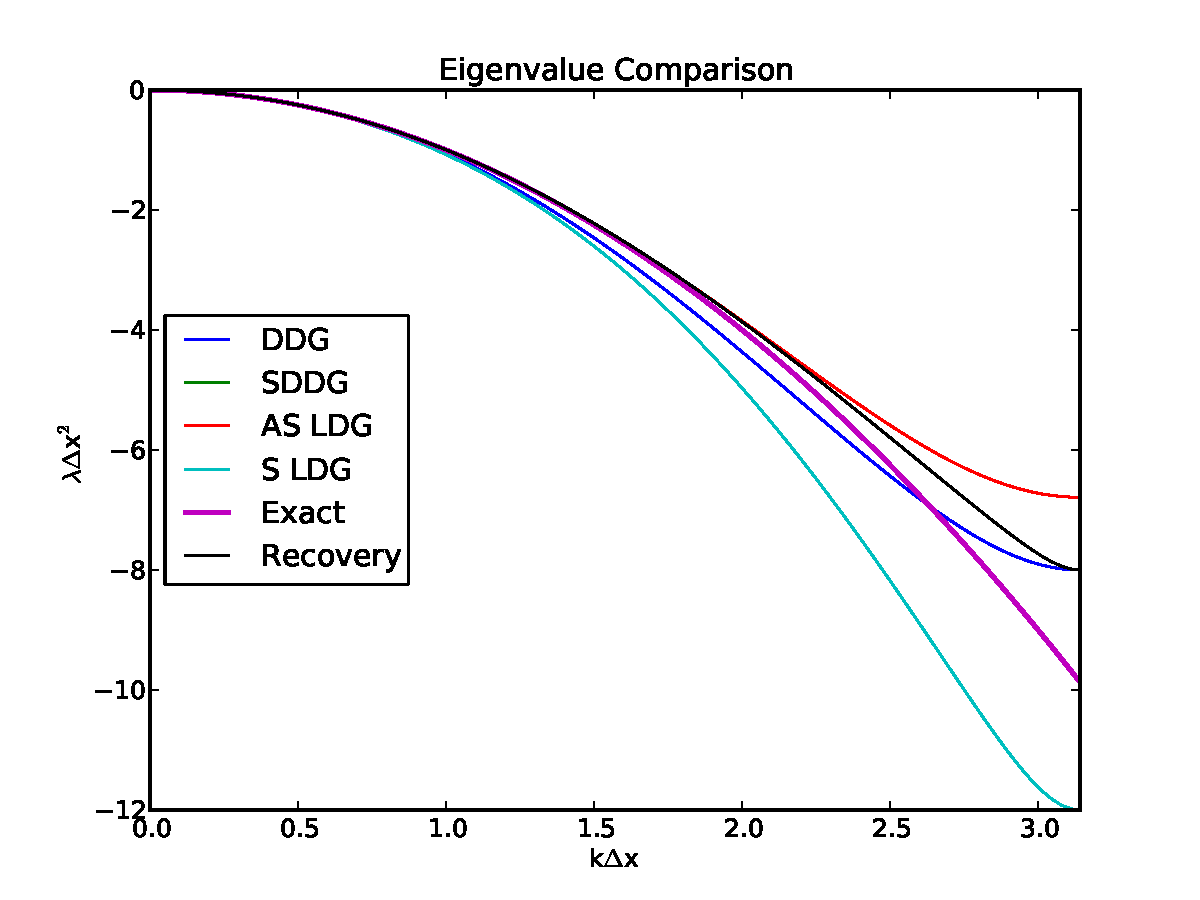
\includegraphics[width=0.75\textwidth]{compareDiffusionSchemes.pdf}
  \end{figure}
\end{frame}

\end{document}

